\documentclass[12pt]{scrartcl}


\usepackage{epsfig,amssymb}

\usepackage{xcolor}
\usepackage{graphicx}
\usepackage{epstopdf}
\usepackage{multirow}

\definecolor{darkred}{rgb}{0.5,0,0}
\definecolor{darkgreen}{rgb}{0,0.5,0}
\usepackage[pdfusetitle]{hyperref}
\hypersetup{
  letterpaper,
  colorlinks,
  linkcolor=red,
  citecolor=darkgreen,
  menucolor=darkred,
  urlcolor=blue,
  pdfpagemode=none,
}

\usepackage{fullpage}
\usepackage{tikz}
\pagestyle{empty} %
\usepackage{subfigure}

\definecolor{MyDarkBlue}{rgb}{0,0.08,0.45}
\definecolor{MyDarkRed}{rgb}{0.45,0.08,0}
\definecolor{MyDarkGreen}{rgb}{0.08,0.45,0.08}

\definecolor{mintedBackground}{rgb}{0.95,0.95,0.95}
\definecolor{mintedInlineBackground}{rgb}{.90,.90,1}

\usepackage[newfloat=true]{minted}

\setminted{mathescape,
           linenos,
           autogobble,
           frame=none,
           framesep=2mm,
           framerule=0.4pt,
           %label=foo,
           xleftmargin=2em,
           xrightmargin=0em,
           %startinline=true,  %PHP only, allow it to omit the PHP Tags *** with this option, variables using dollar sign in comments are treated as latex math
           numbersep=10pt, %gap between line numbers and start of line
           style=default} %syntax highlighting style, default is "default"

\setmintedinline{bgcolor={mintedBackground}}
%doesn't work with the above workaround:
\setminted{bgcolor={mintedBackground}}
\setminted[text]{bgcolor={mintedBackground},linenos=false,autogobble,xleftmargin=1em}
%\setminted[php]{bgcolor=mintedBackgroundPHP} %startinline=True}
\SetupFloatingEnvironment{listing}{name=Code Sample}
\SetupFloatingEnvironment{listing}{listname=List of Code Samples}

\setlength{\parindent}{0pt} %
\setlength{\parskip}{.25cm}
\newcommand{\comment}[1]{}

\usepackage{amsmath}
\usepackage{algorithm2e}
\SetKwInOut{Input}{input}
\SetKwInOut{Output}{output}
%NOTE: you can embed algorithms in solutions, but they cannot be floating objects; use [H] to make them non-floats

\usepackage{lastpage}

%\usepackage{titling}
\usepackage{fancyhdr}
\renewcommand*{\titlepagestyle}{fancy}
\pagestyle{fancy}
%\fancyhf{}
%\rhead{Computer Science I}
%\lhead{Guides and tutorials}
\renewcommand{\headrulewidth}{0.0pt}
\renewcommand{\footrulewidth}{0.4pt}
\lfoot{\Title\ -- Computer Science I}
\cfoot{~}
\rfoot{\thepage\ / \pageref*{LastPage}}


\makeatletter
\title{Hack 7.0}\let\Title\@title
\subtitle{Computer Science I\\
{\small
\vskip1cm
Department of Computer Science \& Engineering \\
University of Nebraska--Lincoln}
\vskip-1cm}
%\author{Dr.\ Chris Bourke}
\date{~}
\makeatother

\begin{document}

\maketitle

\hrule

\section*{Introduction}

Hack session activities are small weekly programming assignments intended
to get you started on full programming assignments.  Collaboration is allowed
and, in fact, \emph{highly encouraged}.  You may start on the activity before
your hack session, but during the hack session you must either be actively 
working on this activity or \emph{helping others} work on the activity.
You are graded using the same rubric as assignments so documentation, style, 
design and correctness are all important.  

\section*{Exercises}

To get more practice working with arrays, you will write several 
functions that involve operations on arrays.  In particular, implement
the following functions.

\begin{enumerate}

  \item Write a function that, given an integer array and an integer 
  $x$ determines if the array contains $x$ anywhere within the array.
  It should return true if it does, false otherwise.
  
  \mintinline{c}{int contains(const int *arr, int size, int x);}

  \item Write a function that, given an integer array and an integer 
  $x$, determines if the array contains $x$ within the range of the two provided indices $ i\;and\; j $ (including both indices).
  It should return true if it does, false otherwise.

  
  \mintinline{c}{int containsWithin(const int *arr, int size, int x, int i, int j);}
  
  \item Write a function that, given an array of integers, its size and a
  ``new size'' creates a new deep copy of the array.  However, instead of
  its original size, the new array should be of the new size.  If the new
  size is less than the old size, only the first \mintinline{c}{newSize} 
  elements should be copied over.  If the new size is greater than the original
  size, then the new array should be padded out with zeros.
  
  \mintinline{c}{int * paddedCopy(const int *arr, int oldSize, int newSize);}

  \item Write a function that, given an array of integers and its size, 
  reverses the elements in the array.  For example, if the original array
  was \mintinline{c}{[10, 15, 5, 25, 0]} the new array should be 
  \mintinline{c}{[0, 25, 5, 15, 10]}.
  
  \mintinline{c}{void reverse(int *arr, int size);}

  \item Write a similar function that creates and returns a new copy of 
  the given array but with its elements in reverse order. 
  
  \mintinline{c}{int * reverseCopy(const int *arr, int size);}

\end{enumerate}

\subsection*{Image Manipulation}

You'll get more practice with 2-dimensional arrays by writing several
functions to manipulate images.  We've adapted a C image library, the 
``stb'' library, and written several \emph{wrapper functions} to load
and save images.  Wrapper functions are functions that call other
functions but may have some ``glue code'' to make the control flow or
data compatible.  In this case, our wrapper functions convert/translate
the stb library's image representation into an RGB pixel representation.
We've defined a \mintinline{c}{Pixel} structure that holds 3 integer
values one for each of the red, green, and blue color values.  We'll
cover structures in detail later on, but it won't prevent you from working
with them.  

You can declare and use a \mintinline{c}{Pixel} type like you would 
an \mintinline{c}{int} or \mintinline{c}{double}: 

\begin{minted}{c}
//a single pixel:
Pixel p;
//an array of n pixels:
Pixel *p = (Pixel *) malloc(sizeof(Pixel) * n);

//swap two pixels:
Pixel a, b;
...
Pixel temp = a;
a = b;
b = temp;
\end{minted} 

An $h \times w$ (height by width) image can be represented as a two dimensional
array of \mintinline{c}{Pixel} types; in particular: \mintinline{c}{Pixel **image}.
Everything we've covered using two dimensional arrays of \mintinline{c}{int} types
applies to \mintinline{c}{Pixel} types.

We've provided a library of functions to load and save a file (you'll need to 
RTM) and specified several function signatures for functions you need to
implement.  
\begin{itemize}
  \item \mintinline{c}{copyImage()} should produce a deep copy of the given
  image.
  \item \mintinline{c}{flipHorizontal()} should flip the image horizontally
  as depicted in Figure \ref{image:pointersHFlip}.
  
  \begin{figure}[h]  
  \centering
  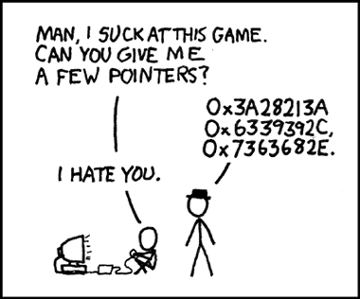
\includegraphics[scale=.50]{hack7.0-files/pointers.png}
  \caption{Original Image}
  \end{figure}
  \begin{figure}[h]  
  \centering
  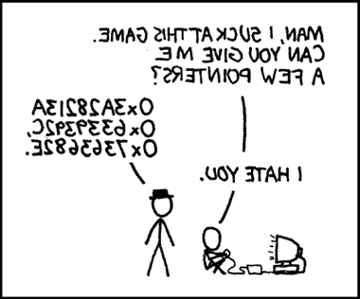
\includegraphics[scale=.50]{hack7.0-files/pointersHFlip}
  \caption{Flipped Horizontally}
  \label{image:pointersHFlip}
  \end{figure}
  \item \mintinline{c}{flipVertical()} should flip the image vertically as
  depicted in Figure \ref{image:pointersVFlip}.
  \begin{figure}[h]  
  \centering
  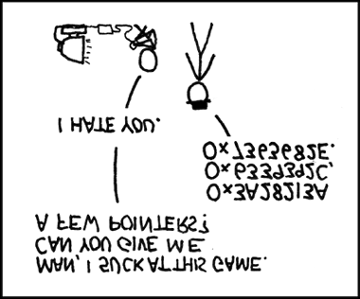
\includegraphics[scale=.50]{hack7.0-files/pointersVFlip}
  \caption{Flipped Vertically}
  \label{image:pointersVFlip}
  \end{figure}
  \item \mintinline{c}{rotateClockwise()} should produce a new image that
  is rotated 90 degrees clockwise.  This function must produce a new image
  because an $h \times w$ sized image that has been rotated will be a 
  $w \times h$ image.  This operation is depicted in Figure \ref{image:pointersRotated}.
  \begin{figure}[h]  
  \centering
  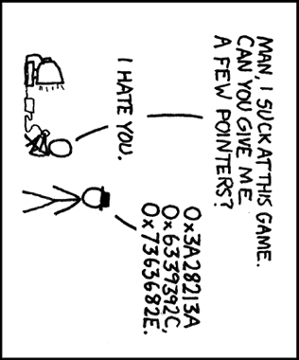
\includegraphics[scale=.50]{hack7.0-files/pointersRotated}
  \caption{Rotated Clockwise}
  \label{image:pointersRotated}
  \end{figure}
\end{itemize}  

\section*{Instructions}




\begin{itemize}

  \item For the warm-up, place all your function prototypes into a file 
  named \mintinline{text}{array_utils.h} and and their definitions in a
  file named \mintinline{text}{array_utils.c}.  You will need to turn
  these in via webhandin.
  
  \item In addition, you'll want to create a main test driver program 
  that demonstrates at least 3 cases per function to verify their output.  
  You need not hand in this test file, however.
  
  \item For the Image Manipulation section, you can use the starter code
  provided here:
  
  \url{https://github.com/cbourke/CSCE155-Hack7.0}
  
  However, you only need to handin \mintinline{text}{imageUtils.h} and
  \mintinline{text}{imageUtils.c}

  \item You should test all your functions with an image (load it, manipulate
  it and save it) of your choice.
  \item As a first step, you should add documentation to all your functions.
  Use this as an opportunity to discuss how the functions should work and
  to \emph{whiteboard} your designs and solutions with other students.
  
  \item You are encouraged to collaborate any number of students 
  before, during, and after your scheduled hack session.  

  \item You may (in fact are encouraged) to define any additional
  ``helper'' functions that may help you.
  \item Include the name(s) of everyone who worked together on
  this activity in your source file's header.

  \item Turn in all of your files via webhandin, making sure that 
  it runs and executes correctly in the webgrader.  Each individual 
  student will need to hand in their own copy and will receive 
  their own individual grade.
\end{itemize}  


\end{document}
